
  
\documentclass[journal,12pt,twocolumn]{IEEEtran}

\usepackage{setspace}
\usepackage{gensymb}
\singlespacing
\usepackage[cmex10]{amsmath}

\usepackage{amsthm}

\usepackage{mathrsfs}
\usepackage{txfonts}
\usepackage{stfloats}
\usepackage{bm}
\usepackage{cite}
\usepackage{cases}
\usepackage{subfig}

\usepackage{longtable}
\usepackage{multirow}

\usepackage{enumitem}
\usepackage{mathtools}
\usepackage{steinmetz}
\usepackage{tikz}
\usepackage{circuitikz}
\usepackage{verbatim}
\usepackage{tfrupee}
\usepackage[breaklinks=true]{hyperref}
\usepackage{graphicx}
\usepackage{tkz-euclide}

\usetikzlibrary{calc,math}
\usepackage{listings}
    \usepackage{color}                                            %%
    \usepackage{array}                                            %%
    \usepackage{longtable}                                        %%
    \usepackage{calc}                                             %%
    \usepackage{multirow}                                         %%
    \usepackage{hhline}                                           %%
    \usepackage{ifthen}                                           %%
    \usepackage{lscape}     
\usepackage{multicol}
\usepackage{chngcntr}

\DeclareMathOperator*{\Res}{Res}
\newtheorem{theorem}{Theorem}[section]
\newtheorem{corollary}{Corollary}[theorem]
\newtheorem{lemma}[theorem]{Lemma}
\newtheorem{definition}{Definition}[section]
\renewcommand\thesection{\arabic{section}}
\renewcommand\thesubsection{\thesection.\arabic{subsection}}
\renewcommand\thesubsubsection{\thesubsection.\arabic{subsubsection}}

\renewcommand\thesectiondis{\arabic{section}}
\renewcommand\thesubsectiondis{\thesectiondis.\arabic{subsection}}
\renewcommand\thesubsubsectiondis{\thesubsectiondis.\arabic{subsubsection}}


\hyphenation{op-tical net-works semi-conduc-tor}
\def\inputGnumericTable{}                                 %%

\lstset{
%language=C,
frame=single, 
breaklines=true,
columns=fullflexible
}
\begin{document}

\newcommand{\BEQA}{\begin{eqnarray}}
\newcommand{\EEQA}{\end{eqnarray}}
\newcommand{\define}{\stackrel{\triangle}{=}}
\bibliographystyle{IEEEtran}
\raggedbottom
\setlength{\parindent}{0pt}
\providecommand{\mbf}{\mathbf}
\providecommand{\pr}[1]{\ensuremath{\Pr\left(#1\right)}}
\providecommand{\qfunc}[1]{\ensuremath{Q\left(#1\right)}}
\providecommand{\sbrak}[1]{\ensuremath{{}\left[#1\right]}}
\providecommand{\lsbrak}[1]{\ensuremath{{}\left[#1\right.}}
\providecommand{\rsbrak}[1]{\ensuremath{{}\left.#1\right]}}
\providecommand{\brak}[1]{\ensuremath{\left(#1\right)}}
\providecommand{\lbrak}[1]{\ensuremath{\left(#1\right.}}
\providecommand{\rbrak}[1]{\ensuremath{\left.#1\right)}}
\providecommand{\cbrak}[1]{\ensuremath{\left\{#1\right\}}}
\providecommand{\lcbrak}[1]{\ensuremath{\left\{#1\right.}}
\providecommand{\rcbrak}[1]{\ensuremath{\left.#1\right\}}}
\theoremstyle{remark}
\newtheorem{rem}{Remark}
\newcommand{\sgn}{\mathop{\mathrm{sgn}}}
\providecommand{\abs}[1]{\vert#1\vert}
\providecommand{\res}[1]{\Res\displaylimits_{#1}} 
\providecommand{\norm}[1]{\lVert#1\rVert}
%\providecommand{\norm}[1]{\lVert#1\rVert}
\providecommand{\mtx}[1]{\mathbf{#1}}
\providecommand{\mean}[1]{E[ #1 ]}
\providecommand{\fourier}{\overset{\mathcal{F}}{ \rightleftharpoons}}
%\providecommand{\hilbert}{\overset{\mathcal{H}}{ \rightleftharpoons}}
\providecommand{\system}{\overset{\mathcal{H}}{ \longleftrightarrow}}
	%\newcommand{\solution}[2]{\textbf{Solution:}{#1}}
\newcommand{\solution}{\noindent \textbf{Solution: }}
\newcommand{\cosec}{\,\text{cosec}\,}
\providecommand{\dec}[2]{\ensuremath{\overset{#1}{\underset{#2}{\gtrless}}}}
\newcommand{\myvec}[1]{\ensuremath{\begin{pmatrix}#1\end{pmatrix}}}
\newcommand{\mydet}[1]{\ensuremath{\begin{vmatrix}#1\end{vmatrix}}}
\numberwithin{equation}{subsection}
\makeatletter
\@addtoreset{figure}{problem}
\makeatother
\let\StandardTheFigure\thefigure
\let\vec\mathbf
\renewcommand{\thefigure}{\theproblem}
\def\putbox#1#2#3{\makebox[0in][l]{\makebox[#1][l]{}\raisebox{\baselineskip}[0in][0in]{\raisebox{#2}[0in][0in]{#3}}}}
     \def\rightbox#1{\makebox[0in][r]{#1}}
     \def\centbox#1{\makebox[0in]{#1}}
     \def\topbox#1{\raisebox{-\baselineskip}[0in][0in]{#1}}
     \def\midbox#1{\raisebox{-0.5\baselineskip}[0in][0in]{#1}}
\vspace{3cm}
\title{GATE Assignment 1}
\author{Adarsh Sai - AI20BTECH11001}
\maketitle
\newpage
\bigskip
\renewcommand{\thefigure}{\theenumi}
\renewcommand{\thetable}{\theenumi}
Download all python codes from 
\begin{lstlisting}
https://github.com/Adarsh541/EE3900/blob/main/Gate1/codes/Gate1.py
\end{lstlisting}

%
Download latex-tikz codes from 
%
\begin{lstlisting}
https://github.com/Adarsh541/EE3900/blob/main/Gate1/Gate1.tex
\end{lstlisting}
\section{Problem(GATE 2021 EC Q4)}
Consider a real-valued base-band signal $x\brak{t}$, band limited to 10 kHz. The Nyquist rate for the signal $y\brak{t} = x\brak{t}x\brak{1+\frac{t}{2}}$ is
\begin{enumerate}
    \item 15 kHz
    \item 30 kHz
    \item 60 kHz
    \item 20 kHz
\end{enumerate}
\section{Solution}
\begin{definition}[Dirac-delta impulse]
\begin{align}
 \delta\brak{t}=
 \begin{cases}
 \infty , & t=0\\
 0, & otherwise
 \end{cases}
\end{align}
\end{definition}
\begin{lemma}[Shifting property of $\delta\brak{t}$]
 If $g\brak{t}$ is a continuous and finite function at $t=a$ then
 \begin{align}
     \int_{-\infty}^{\infty}\delta\brak{t-a}g\brak{t}dt=g\brak{a}
 \end{align}
 We also have
 \begin{align}
     \int_{-\infty}^{\infty}\delta\brak{t-a}\delta\brak{t-b}dt=\delta\brak{a-b}\label{translation}
 \end{align}
\end{lemma}
%%%%%%%%%
\begin{theorem}
Fourier transform of shifted impulse is the complex exponential.
\begin{align}
    G\brak{f}=\mathcal{F}\cbrak{\delta\brak{t-a}}=e^{-i2\pi fa}
\end{align}
\end{theorem}
\begin{proof}
 \begin{align}
     G\brak{f}&=\int_{-\infty}^{\infty}\delta\brak{t-a}e^{-i2\pi ft}dt\\
     &=e^{-i2\pi fa}
 \end{align}
\end{proof}
%%%%%%%%%
\begin{corollary}
Inverse Fourier Transform of the complex exponential must be the shifted impulse. So
\begin{align}
    \mathcal{F}^{-1}\cbrak{e^{-2\pi fa}}&=\int_{-\infty}^{\infty}e^{-2\pi fa}e^{i2\pi ft}df\\
    &=\int_{-\infty}^{\infty}e^{i2\pi f\brak{t-a}}df\\
    &=\int_{-\infty}^{\infty}e^{-i2\pi f\brak{t-a}}df\\
    &=\delta\brak{t-a}
\end{align}
\end{corollary}
%%%%%%%%%
\begin{theorem}
The Fourier transform of $g\brak{t}=e^{i2\pi at}$ is given by 
\begin{align}
    G\brak{f}=\mathcal{F}\cbrak{e^{i2\pi at}}=\delta\brak{f-a}
\end{align}
\begin{proof}
 \begin{align}
     G\brak{f}&=\int_{-\infty}^{\infty}e^{i2\pi at}e^{-i2\pi ft}dt\\
     &=\int_{-\infty}^{\infty}e^{i2\pi t\brak{a-f}}dt\\
     &=\delta\brak{f-a}
 \end{align}
\end{proof}
\end{theorem}
%%%%%%%%
\begin{lemma}[Linearity of Fourier Transform]
\begin{align}
    \mathcal{F}\cbrak{c_1g\brak{t}+c_2h\brak{t}}=c_1\mathcal{F}\cbrak{g\brak{t}}+c_2\mathcal{F}\cbrak{h\brak{t}}
\end{align}
\end{lemma}
%%%%%%%
\begin{lemma}\label{fre}
Let $x\brak{t}$ be a signal, its Fourier Transform  be of the form
\begin{align}
    G_x\brak{f}=c_1\delta\brak{f-a_1A}+c_2\delta\brak{f-a_2A}+...
\end{align}
where $c_i\in \mathbb{C}$ and $a_i\in \mathbb{R}$. 
Then the frequencies present in the signal are $a_jA $ where $a_j\in \mathbb{R}^{+}$
\end{lemma}
%%%%%%%
Let $x\brak{t}=\cos{\brak{2\pi At}}$, where $A=10kHz$.
\begin{align}
  \cos{\brak{2\pi At}}=\frac{e^{i2\pi At}+e^{-i2\pi At}}{2}  
\end{align}
The Fourier transform of $x\brak{t}$ 
\begin{align}
    G_x\brak{f}&=\int_{-\infty}^{\infty}\frac{e^{i2\pi At}+e^{-i2\pi At}}{2}e^{-i2\pi ft}dt\\
    &=\frac{1}{2}\sbrak{\int_{-\infty}^{\infty}e^{-i2\pi t(f-A)}dt+\int_{-\infty}^{\infty}e^{-i2\pi t(A+F)}}\\
    &=\frac{1}{2}\sbrak{\delta\brak{f-A}+\delta\brak{f+A}}
\end{align}
$\therefore$ All the energy of the sinusoidal wave is  entirely localized at the frequencies given by $|f|=A$.
\begin{align}
    y\brak{t}&=\cos{\brak{2\pi At}}\cos{\brak{2\pi A\brak{1+\frac{t}{2}}}}\\
    &=\frac{1}{2}\brak{\cos{\brak{2\pi A+3\pi At}}+\cos{\brak{2\pi A-\pi At}}}\\
    &=\frac{1}{2}\brak{\cos{\brak{3\pi At}}+\cos{\brak{\pi At}}\label{yt}}
\end{align}
Fourier Transform of $y\brak{t}$ is given by
\begin{multline}
    G_y\brak{f}=\frac{1}{4}\sbrak{\delta\brak{f-\frac{3A}{2}}+\delta\brak{f+\frac{3A}{2}}}\\+\frac{1}{4}\sbrak{\delta\brak{f-\frac{A}{2}}+\delta\brak{f+\frac{A}{2}}}
\end{multline}
From lemma $\ref{fre}$ we can conclude that the frequencies present in signal $y\brak{t}$ are $\frac{A}{2},\frac{3A}{2}$
\begin{lemma}{Multiplication property of Fourier Transform}\label{conv}
\begin{align}
    \text{If } x\brak{t} \fourier X\brak{f} \\
    y\brak{t} \fourier Y\brak{f}
\end{align}
Then
\begin{align}
   x\brak{t}y\brak{t} \fourier  X\brak{f} \ast Y\brak{f}
\end{align}
where $\ast$ represents convolution
\end{lemma}
\begin{lemma}
\begin{align}
    \delta\brak{t-t_0}\ast g\brak{t}=g\brak{t-t_0}\label{convdelta}
\end{align}
\end{lemma}
\begin{lemma}{Computing $G_y\brak{f}$ using convolution}
\begin{align}
    x\brak{t}&=\cos{\brak{2\pi At}}\\
    x\brak{t}& \fourier X_1\brak{f}=\frac{1}{2}\sbrak{\delta\brak{f-A}+\delta\brak{f+A}}\\
    x\brak{1+\frac{t}{2}}&=\cos{\brak{\pi At}}\\
    x\brak{1+\frac{t}{2}}& \fourier X_2\brak{f}=\frac{1}{2}\sbrak{\delta\brak{f-\frac{A}{2}}+\delta\brak{f+\frac{A}{2}}}
\end{align}
Using lemma $\ref{conv}$ 
\begin{align}
    G_y\brak{f}&=X_1\brak{f}\ast X_2\brak{f}\\
    &=\brak{\frac{1}{2}\sbrak{\delta\brak{f-A}+\delta\brak{f+A}}}\ast  X_2\brak{f}\\
    &=\frac{1}{2}\cbrak{\delta\brak{f-A}\ast  X_2\brak{f}+\delta\brak{f+A}\ast  X_2\brak{f}}
\end{align}
Using $\eqref{convdelta}$ 
\begin{align}
    G_y\brak{f}=\frac{1}{2}\brak{X_2\brak{f-A}+X_2\brak{f+A}}
\end{align}
\begin{multline}
    G_y\brak{f}=\frac{1}{4}\sbrak{\delta\brak{f-\frac{3A}{2}}+\delta\brak{f+\frac{3A}{2}}}\\+\frac{1}{4}\sbrak{\delta\brak{f-\frac{A}{2}}+\delta\brak{f+\frac{A}{2}}}
\end{multline}
\end{lemma}
\begin{align}
  x\brak{t}&=\cos{\brak{20k\pi t}}\\
    \text{bandwidth of } x\brak{t} &= 10 kHz\\
    x\brak{1+\frac{t}{2}} &= \cos{\brak{20k\pi+10k\pi t}}\\
    \text{bandwidth of } x\brak{1+\frac{t}{2}} &=  5 kHz\\
    \text{from \eqref{yt} } 
    y\brak{t}&= \cos{\brak{30k\pi t}}+\cos{\brak{10k\pi t}}\\
    \text{bandwidth of } y\brak{t} &= \frac{30}{2} kHz\\
    &= 15 kHz
\end{align}
\begin{align}
    \text{Nyquist rate} &= 2 \times \text{maximum frequency}\\
    &= 30 kHz
\end{align}
\begin{figure}[!h]
 \centering
 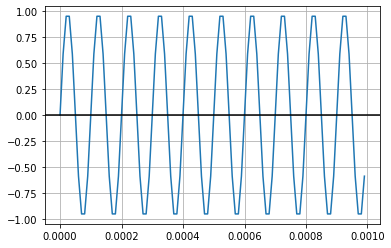
\includegraphics[width=\columnwidth]{x.png}
 \caption{$x\brak{t}$:Sinusoidal signal with freq=10kHz}
\end{figure}
\begin{figure}[!h]
 \centering
 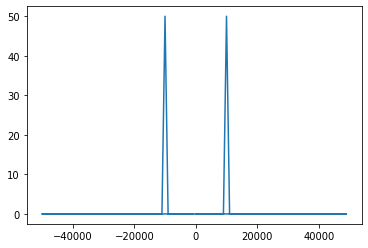
\includegraphics[width=\columnwidth]{xf.png}
 \caption{DFT of $x\brak{t}$. $Bandwidth=10000$}
\end{figure}
\begin{figure}[!h]
 \centering
 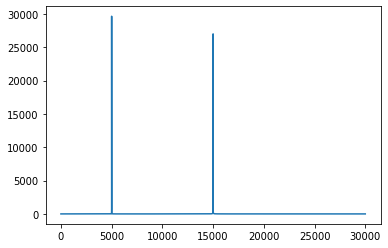
\includegraphics[width=\columnwidth]{four_y.png}
 \caption{DFT of $y\brak{t}$.$Bandwidth=15000$}
\end{figure}
\begin{figure}[!h]
 \centering
 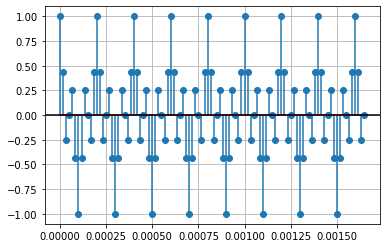
\includegraphics[width=\columnwidth]{stem_y.png}
 \caption{stem plot of $y\brak{t}$ sampled at 60kHz}
\end{figure}
\begin{figure}[!h]
 \centering
 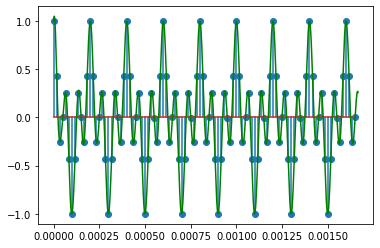
\includegraphics[width=\columnwidth]{interpolation.png}
 \caption{Shannon interpolation of $y\brak{t}$ at 60kHz} 
\end{figure}
\begin{figure}[!h]
 \centering
 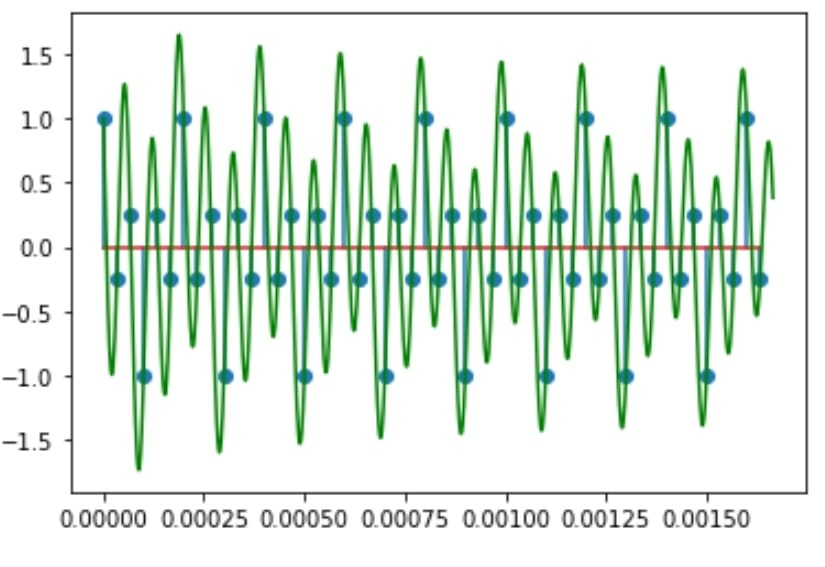
\includegraphics[width=\columnwidth]{int_30k.jpeg}
 \caption{Shannon interpolation of $y\brak{t}$ at 30kHz}
\end{figure}
\end{document}

